\newpage
\null
\thispagestyle{empty}
\newpage
\addcontentsline{toc}{chapter}{2 Corinthians}

% Safely inserts your illustration full-bleed on its own page.
% This completely bypasses the page builder, headers, and geometry bugs!
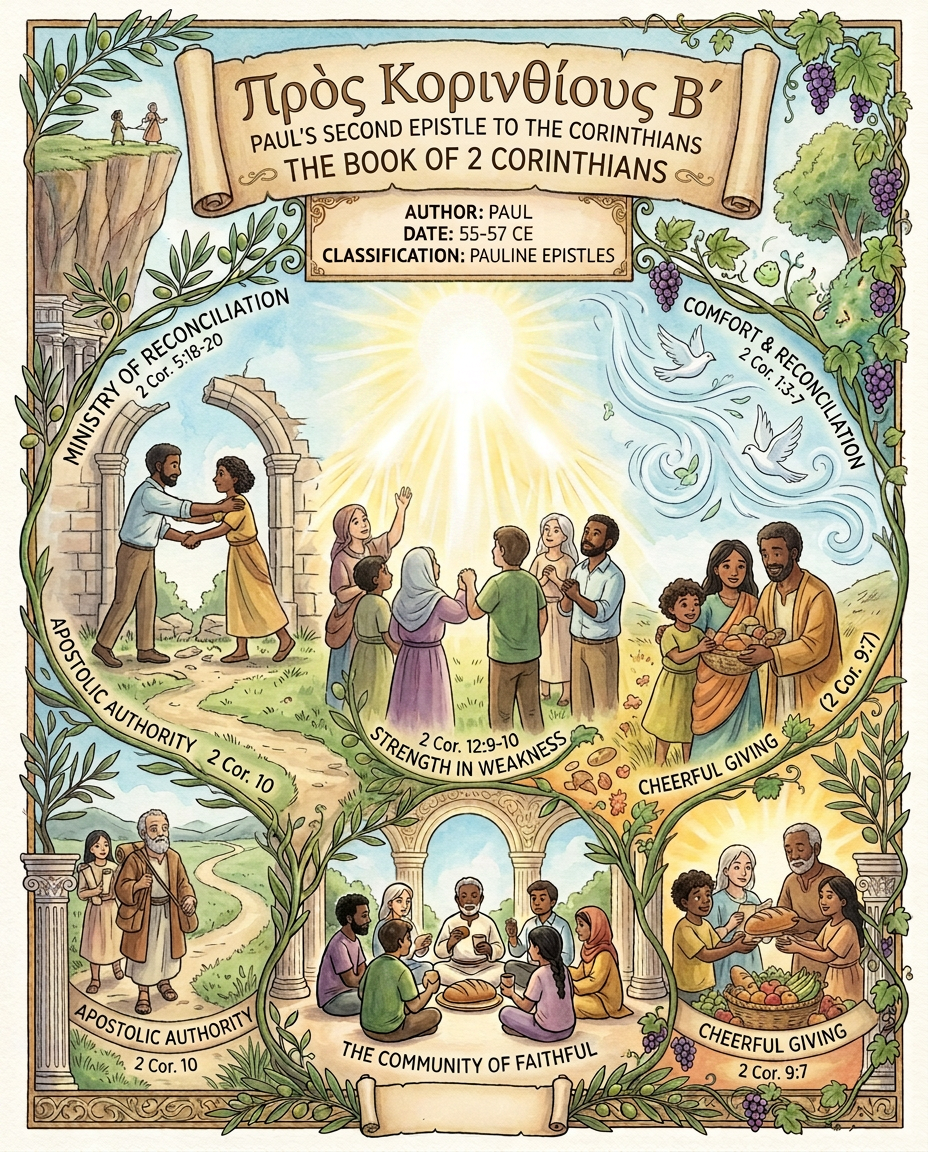
\includepdf[pages=1, fitpaper=false, width=\paperwidth, height=\paperheight, , keepaspectratio=false]{images/divider2/2corinthians2.png}
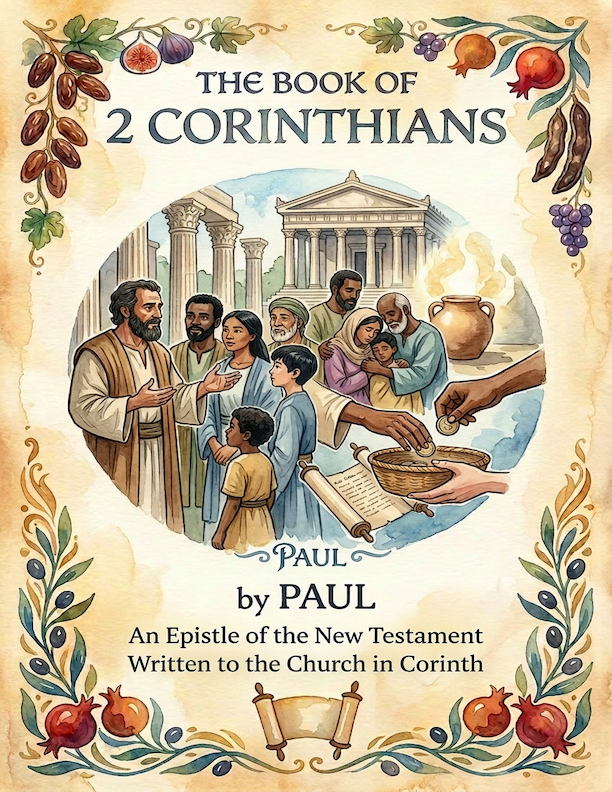
\includepdf[pages=1, fitpaper=false, width=\paperwidth, height=\paperheight, , keepaspectratio=false]{images/divider1/2corinthians.png}

\includepdf[pages=1, fitpaper=false, width=\paperwidth, height=\paperheight, , keepaspectratio=false]{images/8.5x11-Dot-Grid.png}

\includepdf[pages=1, fitpaper=false, width=\paperwidth, height=\paperheight, , keepaspectratio=false]{images/8.5x11-Dot-Grid.png}
\mybook{2 Corinthians}
\vspace{-1.36in}


\mychapter{} \myverse*{}Paul, an emissary of Messiah\footnote{1:1 “Messiah” means “Anointed One”.} Yeshua through the will of God, and Timothy our brother,
to the assembly of God which is at Corinth, with all the holy ones who are in the whole of Achaia:
\myverse{}Grace to you and peace from God our Father and the Lord Yeshua the Messiah.

\myverse{}Blessed be the God and Father of our Lord Yeshua the Messiah, the
Father of mercies and God of all comfort,
\myverse{}who comforts us in all our affliction, that we may be able to comfort those
who are in any affliction, through the comfort with which we ourselves are comforted by God.
\myverse{}For as the sufferings of Messiah abound to us, even so our comfort also abounds
through Messiah.
\myverse{}But if we are afflicted, it is for your comfort and salvation. If we are comforted,
it is for your comfort, which produces in you the patient enduring of the same sufferings which we also
suffer.
\myverse{}Our hope for you is steadfast, knowing that, since you are partakers of the
sufferings, so you are also of the comfort.

\myverse{}For we don’t desire to have you uninformed, brothers,\footnote{1:8 The word for “brothers” here and where context allows may also be correctly translated “brothers
	and sisters” or “siblings.”} concerning our affliction which happened to us in Asia: that we were
weighed down exceedingly, beyond our power, so much that we despaired even of life.
\myverse{}Yes, we ourselves have had the sentence of death within ourselves, that we should
not trust in ourselves, but in God who raises the dead,
\myverse{}who delivered us out of so great a death, and does deliver, on whom we have
set our hope that he will also still deliver us,
\myverse{}you also helping together on our behalf by your supplication; that, for the
gift given to us by means of many, thanks may be given by many persons on your\footnote{1:11 +MT: your; TR and NU: our} behalf.

\myverse{}For our boasting is this: the testimony of our conscience that
in holiness and sincerity of God, not in fleshly wisdom but in the grace of God, we behaved ourselves
in the world, and more abundantly toward you.
\myverse{}For we write no other things to you than what you read or even acknowledge,
and I hope you will acknowledge to the end—
\myverse{}as also you acknowledged us in part—that we are your boasting, even as you
also are ours, in the day of our Lord Yeshua.

\myverse{}In this confidence, I was determined to come first to you, that
you might have a second benefit,
\myverse{}and by you to pass into Macedonia, and again from Macedonia to come to you,
and to be sent forward by you on my journey to Judea.
\myverse{}When I therefore planned this, did I show fickleness? Or the things that I
plan, do I plan according to the flesh, that with me there should be the “Yes, yes” and the “No, no?”
\myverse{}But as God is faithful, our word toward you was not “Yes and no.”
\myverse{}For the Son of God, Yeshua the Messiah, who was preached among you by us—by
me, Silvanus, and Timothy—was not “Yes and no,” but in him is “Yes.”
\myverse{}For however many are the promises of God, in him is the “Yes.” Therefore also
through him is the “Amen”, to the glory of God through us.

\myverse{}Now he who establishes us with you in Messiah and anointed us
is God,
\myverse{}who also sealed us and gave us the down payment of the Spirit in our hearts.

\myverse{}But I call God for a witness to my soul, that to spare you, I
didn’t come to Corinth.
\myverse{}We don’t control your faith, but are fellow workers with you for your joy.
For you stand firm in faith.


% 2 CORINTHIANS 2
\mychapter{} \myverse*{}But I determined this for myself, that I would not come to you
again in sorrow.
\myverse{}For if I make you grieve, then who will make me glad but he who is made to grieve
by me?
\myverse{}And I wrote this very thing to you, so that when I came, I wouldn’t have sorrow
from them of whom I ought to rejoice; having confidence in you all that my joy would be shared by all
of you.
\myverse{}For out of much affliction and anguish of heart I wrote to you with many tears,
not that you should be made to grieve, but that you might know the love that I have so abundantly for
you.

\myverse{}But if any has caused sorrow, he has caused sorrow not to me, but
in part (that I not press too heavily) to you all.
\myverse{}This punishment which was inflicted by the many is sufficient for such a one;
\myverse{}so that, on the contrary, you should rather forgive him and comfort him, lest
by any means such a one should be swallowed up with his excessive sorrow.
\myverse{}Therefore I beg you to confirm your love toward him.
\myverse{}For to this end I also wrote, that I might know the proof of you, whether you
are obedient in all things.
\myverse{}Now I also forgive whomever you forgive anything. For if indeed I have forgiven
anything, I have forgiven that one for your sakes in the presence of Messiah,
\myverse{}that no advantage may be gained over us by Satan, for we are not ignorant
of his schemes.

\myverse{}Now when I came to Troas for the Good News of Messiah, and when
a door was opened to me in the Lord,
\myverse{}I had no relief for my spirit, because I didn’t find Titus my brother, but
taking my leave of them, I went out into Macedonia.

\myverse{}Now thanks be to God who always leads us in triumph in Messiah,
and reveals through us the sweet aroma of his knowledge in every place.
\myverse{}For we are a sweet aroma of Messiah to God in those who are being saved and
in those who perish:
\myverse{}to the one a stench from death to death, to the other a sweet aroma from life
to life. Who is sufficient for these things?
\myverse{}For we are not as so many, peddling the word of God. But as of sincerity,
but as of God, in the sight of God, we speak in Messiah.


% 2 CORINTHIAN 3
\mychapter{} \myverse*{}Are we beginning again to commend ourselves? Or do we need, as
do some, letters of commendation to you or from you?
\myverse{}You are our letter, written in our hearts, known and read by all men,
\myverse{}being revealed that you are a letter of Messiah, served by us, written not with
ink, but with the Spirit of the living God; not in tablets of stone, but in tablets that are hearts of
flesh.

\myverse{}Such confidence we have through Messiah toward God,
\myverse{}not that we are sufficient of ourselves to account anything as from ourselves;
but our sufficiency is from God,
\myverse{}who also made us sufficient as servants of a new covenant, not of the letter
but of the Spirit. For the letter kills, but the Spirit gives life.

\myverse{}But if the service of death, written engraved on stones, came with
glory, so that the children of Israel could not look steadfastly on the face of Moses for the glory of
his face, which was passing away,
\myverse{}won’t service of the Spirit be with much more glory?
\myverse{}For if the service of condemnation has glory, the service of righteousness exceeds
much more in glory.
\myverse{}For most certainly that which has been made glorious has not been made glorious
in this respect, by reason of the glory that surpasses.
\myverse{}For if that which passes away was with glory, much more that which remains
is in glory.

\myverse{}Having therefore such a hope, we use great boldness of speech,
\myverse{}and not as Moses, who put a veil on his face so that the children of Israel
wouldn’t look steadfastly on the end of that which was passing away.
\myverse{}But their minds were hardened, for until this very day at the reading of the
old covenant the same veil remains, because in Messiah it passes away.
\myverse{}But to this day, when Moses is read, a veil lies on their heart.
\myverse{}But whenever someone turns to the Lord, the veil is taken away.
\myverse{}Now the Lord is the Spirit; and where the Spirit of the Lord is, there is
liberty.
\myverse{}But we all, with unveiled face seeing the glory of the Lord as in a mirror,
are transformed into the same image from glory to glory, even as from the Lord, the Spirit.


% 2 CORINTHIANS 4
\mychapter{} \myverse*{}Therefore, seeing we have this ministry, even as we obtained mercy,
we don’t faint.
\myverse{}But we have renounced the hidden things of shame, not walking in craftiness
nor handling the word of God deceitfully, but by the manifestation of the truth commending ourselves to
every man’s conscience in the sight of God.
\myverse{}Even if our Good News is veiled, it is veiled in those who are dying,
\myverse{}in whom the god of this world has blinded the minds of the unbelieving, that
the light of the Good News of the glory of Messiah, who is the image of God, should not dawn on them.
\myverse{}For we don’t proclaim ourselves, but Messiah Yeshua as Lord, and ourselves as
your servants for Yeshua’s sake,
\myverse{}seeing it is God who said, “Light will shine out of darkness,”\footnote{4:6 Genesis 1:3} who has shone in our hearts to give the light of
the knowledge of the glory of God in the face of Yeshua the Messiah.

\myverse{}But we have this treasure in clay vessels, that the exceeding greatness
of the power may be of God and not from ourselves.
\myverse{}We are pressed on every side, yet not crushed; perplexed, yet not to despair;
\myverse{}pursued, yet not forsaken; struck down, yet not destroyed;
\myverse{}always carrying in the body the putting to death of the Lord Yeshua, that
the life of Yeshua may also be revealed in our body.
\myverse{}For we who live are always delivered to death for Yeshua’s sake, that the
life also of Yeshua may be revealed in our mortal flesh.
\myverse{}So then death works in us, but life in you.

\myverse{}But having the same spirit of faith, according to that which
is written, “I believed, and therefore I spoke.”\footnote{4:13 Psalms 116:10} We also believe, and therefore we also speak,
\myverse{}knowing that he who raised the Lord Yeshua will raise us also through\footnote{4:14 NU reads
	\textit{with} instead of \textit{through}.} Yeshua, and will present us with you.
\myverse{}For all things are for your sakes, that the grace, being multiplied through
the many, may cause the thanksgiving to abound to the glory of God.

\myverse{}Therefore we don’t faint, but though our outward person is decaying,
yet our inward person is renewed day by day.
\myverse{}For our light affliction, which is for the moment, works for us more and more
exceedingly an eternal weight of glory,
\myverse{}while we don’t look at the things which are seen, but at the things which
are not seen. For the things which are seen are temporal, but the things which are not seen are eternal.


% 2 CORINTHIANS 5
\mychapter{} \myverse*{}For we know that if the earthly house of our tent is dissolved,
we have a building from God, a house not made with hands, eternal, in the heavens.
\myverse{}For most certainly in this we groan, longing to be clothed with our habitation
which is from heaven,
\myverse{}if indeed being clothed, we will not be found naked.
\myverse{}For indeed we who are in this tent do groan, being burdened, not that we desire
to be unclothed, but that we desire to be clothed, that what is mortal may be swallowed up by life.
\myverse{}Now he who made us for this very thing is God, who also gave to us the down
payment of the Spirit.

\myverse{}Therefore we are always confident and know that while we are at
home in the body, we are absent from the Lord;
\myverse{}for we walk by faith, not by sight.
\myverse{}We are courageous, I say, and are willing rather to be absent from the body
and to be at home with the Lord.
\myverse{}Therefore also we make it our aim, whether at home or absent, to be well pleasing
to him.
\myverse{}For we must all be revealed before the judgment seat of Messiah that each
one may receive the things in the body according to what he has done, whether good or bad.

\myverse{}Knowing therefore the fear of the Lord, we persuade men, but
we are revealed to God, and I hope that we are revealed also in your consciences.
\myverse{}For we are not commending ourselves to you again, but speak as giving you
occasion of boasting on our behalf, that you may have something to answer those who boast in appearance
and not in heart.
\myverse{}For if we are beside ourselves, it is for God. Or if we are of sober mind,
it is for you.
\myverse{}For the love of Messiah compels us; because we judge thus: that one died for
all, therefore all died.
\myverse{}He died for all, that those who live should no longer live to themselves,
but to him who for their sakes died and rose again.

\myverse{}Therefore we know no one according to the flesh from now on.
Even though we have known Messiah according to the flesh, yet now we know him so no more.
\myverse{}Therefore if anyone is in Messiah, he is a new creation. The old things have
passed away. Behold,\footnote{5:17 “Behold”, from “ἰδοὺ”, means look at, take notice, observe, see, or gaze at. It is often used
	as an interjection.} all things have become new.
\myverse{}But all things are of God, who reconciled us to himself through Yeshua the Messiah,
and gave to us the ministry of reconciliation;
\myverse{}namely, that God was in Messiah reconciling the world to himself, not reckoning
to them their trespasses, and having committed to us the word of reconciliation.

\myverse{}We are therefore ambassadors on behalf of Messiah, as though
God were entreating by us: we beg you on behalf of Messiah, be reconciled to God.
\myverse{}For him who knew no sin he made to be sin on our behalf, so that in him we
might become the righteousness of God.


% 2 CORINTHIANS 6
\mychapter{} \myverse*{}Working together, we entreat also that you do not receive the grace
of God in vain.
\myverse{}For he says,

\quad\quad “At an acceptable time I listened to you.

In a day of salvation I helped you.”\footnote{6:2 Isaiah 49:8}

Behold, now is the acceptable time. Behold, now is the day of salvation.
\myverse{}We give no occasion of stumbling in anything, that our service may not be blamed,
\myverse{}but in everything commending ourselves as servants of God: in great endurance,
in afflictions, in hardships, in distresses,
\myverse{}in beatings, in imprisonments, in riots, in labors, in watchings, in fastings,
\myverse{}in pureness, in knowledge, in perseverance, in kindness, in the Holy Spirit,
in sincere love,
\myverse{}in the word of truth, in the power of God, by the armor of righteousness on
the right hand and on the left,
\myverse{}by glory and dishonor, by evil report and good report, as deceivers and yet
true,
\myverse{}as unknown and yet well known, as dying and behold—we live, as punished and
not killed,
\myverse{}as sorrowful yet always rejoicing, as poor yet making many rich, as having
nothing and yet possessing all things.

\myverse{}Our mouth is open to you, Corinthians. Our heart is enlarged.
\myverse{}You are not restricted by us, but you are restricted by your own affections.
\myverse{}Now in return—I speak as to my children—you also open your hearts.

\myverse{}Don’t be unequally yoked with unbelievers, for what fellowship
do righteousness and iniquity have? Or what fellowship does light have with darkness?
\myverse{}What agreement does Messiah have with Belial? Or what portion does a believer
have with an unbeliever?
\myverse{}What agreement does a temple of God have with idols? For you are a temple
of the living God. Even as God said, “I will dwell in them and walk in them. I will be their God and they
will be my people.”\footnote{6:16 Leviticus 26:12;
	Jeremiah 32:38;
	Ezekiel 37:27}
\myverse{}Therefore

“ ‘Come out from among them,

and be separate,’ says the Lord.

‘Touch no unclean thing.

I will receive you.\footnote{6:17 Isaiah 52:11;
	Ezekiel 20:34,41}

\myverse{}I will be to you a Father.

You will be to me sons and daughters,’

says the Lord Almighty.”\footnote{6:18 2 Samuel 7:14;
	7:8}


%2 CORINTHIANS 7
\mychapter{} \myverse*{}Having therefore these promises, beloved, let’s cleanse ourselves
from all defilement of flesh and spirit, perfecting holiness in the fear of God.

\myverse{}Open your hearts to us. We wronged no one. We corrupted no one.
We took advantage of no one.
\myverse{}I say this not to condemn you, for I have said before that you are in our hearts
to die together and live together.
\myverse{}Great is my boldness of speech toward you. Great is my boasting on your behalf.
I am filled with comfort. I overflow with joy in all our affliction.

\myverse{}For even when we had come into Macedonia, our flesh had no relief,
but we were afflicted on every side. Fightings were outside. Fear was inside.
\myverse{}Nevertheless, he who comforts the lowly, God, comforted us by the coming of
Titus,
\myverse{}and not by his coming only, but also by the comfort with which he was comforted
in you while he told us of your longing, your mourning, and your zeal for me, so that I rejoiced still
more.

\myverse{}For though I grieved you with my letter, I do not regret it, though
I did regret it. For I see that my letter made you grieve, though just for a while.
\myverse{}I now rejoice, not that you were grieved, but that you were grieved to repentance.
For you were grieved in a godly way, that you might suffer loss by us in nothing.
\myverse{}For godly sorrow produces repentance leading to salvation, which brings no
regret. But the sorrow of the world produces death.
\myverse{}For behold, this same thing, that you were grieved in a godly way, what earnest
care it worked in you. Yes, what defense, indignation, fear, longing, zeal, and vindication! In everything
you demonstrated yourselves to be pure in the matter.
\myverse{}So although I wrote to you, I wrote not for his cause that did the wrong,
nor for his cause that suffered the wrong, but that your earnest care for us might be revealed in you
in the sight of God.
\myverse{}Therefore we have been comforted. In our comfort we rejoiced the more exceedingly
for the joy of Titus, because his spirit has been refreshed by you all.
\myverse{}For if in anything I have boasted to him on your behalf, I was not disappointed.
But as we spoke all things to you in truth, so our glorying also which I made before Titus was found to
be truth.
\myverse{}His affection is more abundantly toward you, while he remembers all of your
obedience, how with fear and trembling you received him.
\myverse{}I rejoice that in everything I am confident concerning you.


% 2 CORINTHIANS 8
\mychapter{} \myverse*{}Moreover, brothers, we make known to you the grace of God which
has been given in the assemblies of Macedonia,
\myverse{}how in a severe ordeal of affliction, the abundance of their joy and their deep
poverty abounded to the riches of their generosity.
\myverse{}For according to their power, I testify, yes and beyond their power, they gave
of their own accord,
\myverse{}begging us with much entreaty to receive this grace and the fellowship in the
service to the holy ones.
\myverse{}This was not as we had expected, but first they gave their own selves to the
Lord, and to us through the will of God.
\myverse{}So we urged Titus, that as he had made a beginning before, so he would also
complete in you this grace.
\myverse{}But as you abound in everything—in faith, utterance, knowledge, all earnestness,
and in your love to us—see that you also abound in this grace.

\myverse{}I speak not by way of commandment, but as proving through the earnestness
of others the sincerity also of your love.
\myverse{}For you know the grace of our Lord Yeshua the Messiah, that though he was rich,
yet for your sakes he became poor, that you through his poverty might become rich.
\myverse{}I give advice in this: it is expedient for you who were the first to start
a year ago, not only to do, but also to be willing.
\myverse{}But now complete the doing also, that as there was the readiness to be willing,
so there may be the completion also out of your ability.
\myverse{}For if the readiness is there, it is acceptable according to what you have,
not according to what you don’t have.
\myverse{}For this is not that others may be eased and you distressed,
\myverse{}but for equality. Your abundance at this present time supplies their lack,
that their abundance also may become a supply for your lack, that there may be equality.
\myverse{}As it is written, “He who gathered much had nothing left over, and he who
gathered little had no lack.”\footnote{8:15 Exodus 16:18}

\myverse{}But thanks be to God, who puts the same earnest care for you
into the heart of Titus.
\myverse{}For he indeed accepted our exhortation, but being himself very earnest, he
went out to you of his own accord.
\myverse{}We have sent together with him the brother whose praise in the Good News is
known throughout all the assemblies.
\myverse{}Not only so, but he was also appointed by the assemblies to travel with us
in this grace, which is served by us to the glory of the Lord himself, and to show our readiness.
\myverse{}We are avoiding this, that any man should blame us concerning this abundance
which is administered by us.
\myverse{}Having regard for honorable things, not only in the sight of the Lord, but
also in the sight of men.
\myverse{}We have sent with them our brother whom we have many times proved earnest
in many things, but now much more earnest, by reason of the great confidence which he has in you.
\myverse{}As for Titus, he is my partner and fellow worker for you. As for our brothers,
they are the emissaries of the assemblies, the glory of Messiah.
\myverse{}Therefore show the proof of your love to them before the assemblies, and of
our boasting on your behalf.


%2 CORINTHIANS 9
\mychapter{} \myverse*{}It is indeed unnecessary for me to write to you concerning the
service to the holy ones,
\myverse{}for I know your readiness, of which I boast on your behalf to those of Macedonia,
that Achaia has been prepared for the past year. Your zeal has stirred up very many of them.
\myverse{}But I have sent the brothers so that our boasting on your behalf may not be
in vain in this respect, that, just as I said, you may be prepared,
\myverse{}lest by any means, if anyone from Macedonia comes there with me and finds you
unprepared, we (to say nothing of you) would be disappointed in this confident boasting.
\myverse{}I thought it necessary therefore to entreat the brothers that they would go
before to you and arrange ahead of time the generous gift that you promised before, that the same might
be ready as a matter of generosity, and not of greediness.

\myverse{}Remember this: he who sows sparingly will also reap sparingly.
He who sows bountifully will also reap bountifully.
\myverse{}Let each man give according as he has determined in his heart, not grudgingly
or under compulsion, for God loves a cheerful giver.
\myverse{}And God is able to make all grace abound to you, that you, always having all
sufficiency in everything, may abound to every good work.
\myverse{}As it is written,

“He has scattered abroad. He has given to the poor.

His righteousness remains forever.”\footnote{9:9 Psalms 112:9}

\myverse{}Now may he who supplies seed to the sower and bread for food,
supply and multiply your seed for sowing, and increase the fruits of your righteousness,
\myverse{}you being enriched in everything for all generosity, which produces thanksgiving
to God through us.
\myverse{}For this service of giving that you perform not only makes up for lack among
the holy ones, but abounds also through much giving of thanks to God,
\myverse{}seeing that through the proof given by this service, they glorify God for
the obedience of your confession to the Good News of Messiah and for the generosity of your contribution
to them and to all,
\myverse{}while they themselves also, with supplication on your behalf, yearn for you
by reason of the exceeding grace of God in you.
\myverse{}Now thanks be to God for his unspeakable gift!


% 2 CORINTHIANS 10
\mychapter{} \myverse*{}Now I Paul, myself, entreat you by the humility and gentleness
of Messiah, I who in your presence am lowly among you, but being absent am bold toward you.
\myverse{}Yes, I beg you that I may not, when present, show courage with the confidence
with which I intend to be bold against some, who consider us to be walking according to the flesh.
\myverse{}For though we walk in the flesh, we don’t wage war according to the flesh;
\myverse{}for the weapons of our warfare are not of the flesh, but mighty before God
to the throwing down of strongholds,
\myverse{}throwing down imaginations and every high thing that is exalted against the
knowledge of God and bringing every thought into captivity to the obedience of Messiah,
\myverse{}and being in readiness to avenge all disobedience when your obedience is made
full.

\myverse{}Do you look at things only as they appear in front of your face?
If anyone trusts in himself that he is Messiah’s, let him consider this again with himself, that even
as he is Messiah’s, so we also are Messiah’s.
\myverse{}For even if I boast somewhat abundantly concerning our authority, which the
Lord gave for building you up and not for casting you down, I will not be ashamed,
\myverse{}that I may not seem as if I desire to terrify you by my letters.
\myverse{}For, “His letters”, they say, “are weighty and strong, but his bodily presence
is weak, and his speech is despised.”
\myverse{}Let such a person consider this, that what we are in word by letters when
we are absent, such are we also in deed when we are present.

\myverse{}For we are not bold to number or compare ourselves with some
of those who commend themselves. But they themselves, measuring themselves by themselves, and comparing
themselves with themselves, are without understanding.
\myverse{}But we will not boast beyond proper limits, but within the boundaries with
which God appointed to us, which reach even to you.
\myverse{}For we don’t stretch ourselves too much, as though we didn’t reach to you.
For we came even as far as to you with the Good News of Messiah,
\myverse{}not boasting beyond proper limits in other men’s labors, but having hope
that as your faith grows, we will be abundantly enlarged by you in our sphere of influence,
\myverse{}so as to proclaim the Good News even to the parts beyond you, not to boast
in what someone else has already done.
\myverse{}But “he who boasts, let him boast in the Lord.”\footnote{10:17 Jeremiah 9:24
}
\myverse{}For it isn’t he who commends himself who is approved, but whom the Lord commends.


% 2 CORINTHIANS 11
\mychapter{} \myverse*{}I wish that you would bear with me in a little foolishness, but
indeed you do bear with me.
\myverse{}For I am jealous over you with a godly jealousy. For I promised you in marriage
to one husband, that I might present you as a pure virgin to Messiah.
\myverse{}But I am afraid that somehow, as the serpent deceived Havah in his craftiness,
so your minds might be corrupted from the simplicity that is in Messiah.
\myverse{}For if he who comes preaches another Yeshua whom we didn’t proclaim, or if
you receive a different spirit which you didn’t receive, or a different “good news” which you didn’t accept,
you put up with that well enough.
\myverse{}For I reckon that I am not at all behind the very best emissaries.
\myverse{}But though I am unskilled in speech, yet I am not unskilled in knowledge. No,
in every way we have been revealed to you in all things.

\myverse{}Or did I commit a sin in humbling myself that you might be exalted,
because I preached to you God’s Good News free of charge?
\myverse{}I robbed other assemblies, taking wages from them that I might serve you.
\myverse{}When I was present with you and was in need, I wasn’t a burden on anyone, for
the brothers, when they came from Macedonia, supplied the measure of my need. In everything I kept myself
from being burdensome to you, and I will continue to do so.
\myverse{}As the truth of Messiah is in me, no one will stop me from this boasting
in the regions of Achaia.
\myverse{}Why? Because I don’t love you? God knows.

\myverse{}But what I do, that I will continue to do, that I may cut off
opportunity from those who desire an opportunity, that in which they boast, they may be recognized just
like us.
\myverse{}For such men are false emissaries, deceitful workers, masquerading as Messiah’s
emissaries.
\myverse{}And no wonder, for even Satan masquerades as an angel of light.
\myverse{}It is no great thing therefore if his servants also masquerade as servants
of righteousness, whose end will be according to their works.

\myverse{}I say again, let no one think me foolish. But if so, yet receive
me as foolish, that I also may boast a little.
\myverse{}That which I speak, I don’t speak according to the Lord, but as in foolishness,
in this confidence of boasting.
\myverse{}Seeing that many boast after the flesh, I will also boast.
\myverse{}For you bear with the foolish gladly, being wise.
\myverse{}For you bear with a man if he brings you into bondage, if he devours you,
if he takes you captive, if he exalts himself, or if he strikes you on the face.
\myverse{}To my shame, I speak as though we had been weak. Yet in whatever way anyone
is bold (I speak in foolishness), I am bold also.
\myverse{}Are they Hebrews? So am I. Are they Israelites? So am I. Are they the offspring\footnote{11:22 or, seed} of Abraham? So am I.
\myverse{}Are they servants of Messiah? (I speak as one beside himself.) I am more
so: in labors more abundantly, in prisons more abundantly, in stripes above measure, and in deaths often.
\myverse{}Five times I received forty stripes minus one from the Jews.
\myverse{}Three times I was beaten with rods. Once I was stoned. Three times I suffered
shipwreck. I have been a night and a day in the deep.
\myverse{}I have been in travels often, perils of rivers, perils of robbers, perils
from my countrymen, perils from the Gentiles, perils in the city, perils in the wilderness, perils in
the sea, perils among false brothers;
\myverse{}in labor and travail, in watchings often, in hunger and thirst, in fastings
often, and in cold and nakedness.

\myverse{}Besides those things that are outside, there is that which presses
on me daily: anxiety for all the assemblies.
\myverse{}Who is weak, and I am not weak? Who is caused to stumble, and I don’t burn
with indignation?

\myverse{}If I must boast, I will boast of the things that concern my
weakness.
\myverse{}The God and Father of the Lord Yeshua the Messiah, he who is blessed forever
more, knows that I don’t lie.
\myverse{}In Damascus the governor under King Aretas guarded the Damascenes’ city,
desiring to arrest me.
\myverse{}I was let down in a basket through a window by the wall, and escaped his
hands.


% 2 CORINTHIANS 12
\mychapter{} \myverse*{}It is doubtless not profitable for me to boast, but I will come
to visions and revelations of the Lord.
\myverse{}I know a man in Messiah who was caught up into the third heaven fourteen years
ago—whether in the body, I don’t know, or whether out of the body, I don’t know; God knows.
\myverse{}I know such a man (whether in the body, or outside of the body, I don’t know;
God knows),
\myverse{}how he was caught up into Paradise and heard unspeakable words, which it is
not lawful for a man to utter.
\myverse{}On behalf of such a one I will boast, but on my own behalf I will not boast,
except in my weaknesses.
\myverse{}For if I would desire to boast, I will not be foolish; for I will speak the
truth. But I refrain, so that no man may think more of me than that which he sees in me or hears from
me.
\myverse{}By reason of the exceeding greatness of the revelations, that I should not
be exalted excessively, a thorn in the flesh was given to me: a messenger of Satan to torment me, that
I should not be exalted excessively.
\myverse{}Concerning this thing, I begged the Lord three times that it might depart from
me.
\myverse{}He has said to me,
\textcolor{crimson}{“My grace is sufficient for you, for my power is made perfect in weakness.”} Most gladly therefore
I will rather glory in my weaknesses, that the power of Messiah may rest on me.

\myverse{}Therefore I take pleasure in weaknesses, in injuries, in necessities,
in persecutions, and in distresses, for Messiah’s sake. For when I am weak, then am I strong.
\myverse{}I have become foolish in boasting. You compelled me, for I ought to have
been commended by you, for I am in no way inferior to the very best emissaries, though I am nothing.
\myverse{}Truly the signs of an emissary were worked among you in all perseverance,
in signs and wonders and mighty works.
\myverse{}For what is there in which you were made inferior to the rest of the assemblies,
unless it is that I myself was not a burden to you? Forgive me this wrong!

\myverse{}Behold, this is the third time I am ready to come to you, and
I will not be a burden to you; for I seek not your possessions, but you. For the children ought not to
save up for the parents, but the parents for the children.
\myverse{}I will most gladly spend and be spent for your souls. If I love you more
abundantly, am I loved the less?
\myverse{}Even so, I myself didn’t burden you. But you might say that being crafty,
I caught you with deception.
\myverse{}Did I take advantage of you by anyone of those whom I have sent to you?
\myverse{}I exhorted Titus, and I sent the brother with him. Did Titus take any advantage
of you? Didn’t we walk in the same spirit? Didn’t we walk in the same steps?

\myverse{}Again, do you think that we are excusing ourselves to you? In
the sight of God we speak in Messiah. But all things, beloved, are for your edifying.
\myverse{}For I am afraid that perhaps when I come, I might find you not the way I
want to, and that I might be found by you as you don’t desire, that perhaps there would be strife, jealousy,
outbursts of anger, factions, slander, whisperings, proud thoughts, or riots,
\myverse{}that again when I come my God would humble me before you, and I would mourn
for many of those who have sinned before now, and not repented of the uncleanness, sexual immorality,
and lustfulness which they committed.


% 2 CORINTHIANS 13
\mychapter{} \myverse*{}This is the third time I am coming to you. “At the mouth of two
or three witnesses shall every word be established.”\footnote{13:1 Deuteronomy 19:15}
\myverse{}I have warned previously, and I warn again, as when I was present the second
time, so now, being absent, I write to those who have sinned before now and to all the rest that if I
come again, I will not spare,
\myverse{}seeing that you seek a proof of Messiah who speaks in me who is not weak, but
is powerful in you.
\myverse{}For he was crucified through weakness, yet he lives through the power of God.
For we also are weak in him, but we will live with him through the power of God toward you.

\myverse{}Examine your own selves, whether you are in the faith. Test your
own selves. Or don’t you know about your own selves, that Yeshua the Messiah is in you?—unless indeed
you are disqualified.
\myverse{}But I hope that you will know that we aren’t disqualified.

\myverse{}Now I pray to God that you do no evil; not that we may appear
approved, but that you may do that which is honorable, though we may seem to have failed.
\myverse{}For we can do nothing against the truth, but for the truth.
\myverse{}For we rejoice when we are weak and you are strong. We also pray for this:
your becoming perfect.
\myverse{}For this cause I write these things while absent, that I may not deal sharply
when present, according to the authority which the Lord gave me for building up and not for tearing down.

\myverse{}Finally, brothers, rejoice! Be perfected. Be comforted. Be of
the same mind. Live in peace, and the God of love and peace will be with you.
\myverse{}Greet one another with a holy kiss.

\myverse{}All the holy ones greet you.

\myverse{}The grace of the Lord Yeshua the Messiah, God’s love, and the
fellowship of the Holy Spirit be with you all. Amen.



